\documentclass[12pt]{article}
\usepackage{amsmath,amsfonts,amssymb,fullpage,tikz}
\newcommand{\bh}{\bar{h}}
\setlength{\parindent}{0pt}
\setlength{\parskip}{0.6em}
\begin{document}
\begin{center}
{\bf\Large General Relativity --- Final Examination: Answers}
\end{center}

\section*{Question 1}
Under a change of coordinates $x^\mu\to x'^\mu(x)$ the Riemann tensor, being a $(1,3)$ tensor, transforms as
\[
R'^{\mu}{}_{\nu\rho\sigma}=\frac{\partial x'^\mu}{\partial x^\alpha}\frac{\partial x^\beta}{\partial x'^\nu}\frac{\partial x^\gamma}{\partial x'^\rho}\frac{\partial x^\delta}{\partial x'^\sigma}\,R^\alpha{}_{\beta\gamma\delta}.
\]
The Ricci tensor in the new coordinates is obtained by setting $\mu=\rho$ and summing:
\[
R'_{\nu\sigma}=R'^{\rho}{}_{\nu\rho\sigma}
=\frac{\partial x'^\rho}{\partial x^\alpha}\frac{\partial x^\gamma}{\partial x'^\rho}\,
\frac{\partial x^\beta}{\partial x'^\nu}\frac{\partial x^\delta}{\partial x'^\sigma}\,R^\alpha{}_{\beta\gamma\delta}.
\]
By the chain rule, $\dfrac{\partial x^\gamma}{\partial x'^\rho}\dfrac{\partial x'^\rho}{\partial x^\alpha}=\dfrac{\partial x^\gamma}{\partial x^\alpha}=\delta^\gamma_\alpha$. Hence
\[
R'_{\nu\sigma}=\delta^\gamma_\alpha\frac{\partial x^\beta}{\partial x'^\nu}\frac{\partial x^\delta}{\partial x'^\sigma}R^\alpha{}_{\beta\gamma\delta}
=\frac{\partial x^\beta}{\partial x'^\nu}\frac{\partial x^\delta}{\partial x'^\sigma}R^\alpha{}_{\beta\alpha\delta}
=\frac{\partial x^\beta}{\partial x'^\nu}\frac{\partial x^\delta}{\partial x'^\sigma}R_{\beta\delta},
\]
which is precisely the transformation law of a $(0,2)$ tensor.

\section*{Question 2}
Convention: $\hat\nabla_\mu V^\rho=\partial_\mu V^\rho+\hat\Gamma_{\mu\nu}{}^\rho V^\nu$, $\hat\nabla_\mu \omega_\nu=\partial_\mu\omega_\nu-\hat\Gamma_{\mu\nu}{}^\rho\omega_\rho$. Write $\hat\Gamma_{\mu\nu}{}^\rho=\Gamma_{\mu\nu}{}^\rho+K_{\mu\nu}{}^\rho$ with $K_{\mu\nu}{}^\rho=\tfrac1{12}g^{\rho\sigma}H_{\mu\nu\sigma}=\tfrac1{12}H_{\mu\nu}{}^\rho$. (The difference of two connections is a tensor, so $\hat\Gamma$ is indeed a connection.)

\textbf{a) Torsion.} The torsion tensor is
\[
T_{\mu\nu}{}^\rho=\hat\Gamma_{\mu\nu}{}^\rho-\hat\Gamma_{\nu\mu}{}^\rho
=\underbrace{\Gamma_{\mu\nu}{}^\rho-\Gamma_{\nu\mu}{}^\rho}_{=0}+\tfrac1{12}g^{\rho\sigma}(H_{\mu\nu\sigma}-H_{\nu\mu\sigma})
=\tfrac16 g^{\rho\sigma}H_{\mu\nu\sigma}=\tfrac16H_{\mu\nu}{}^\rho .
\]
This is non-zero whenever $H\neq0$, so $\hat\Gamma$ is \emph{not} torsion-free (the torsion is totally antisymmetric, $T_{\mu\nu\rho}=\tfrac16H_{\mu\nu\rho}$).

\textbf{Metric compatibility.}
\[
\hat\nabla_\mu g_{\nu\lambda}=\partial_\mu g_{\nu\lambda}-\hat\Gamma_{\mu\nu}{}^\sigma g_{\sigma\lambda}-\hat\Gamma_{\mu\lambda}{}^\sigma g_{\nu\sigma}
=\underbrace{\nabla_\mu g_{\nu\lambda}}_{=0\ (\text{Levi-Civita})}-\tfrac1{12}\left(H_{\mu\nu}{}^{\sigma}g_{\sigma\lambda}+H_{\mu\lambda}{}^{\sigma}g_{\nu\sigma}\right).
\]
Since $g^{\sigma\kappa}H_{\mu\nu\kappa}g_{\sigma\lambda}=H_{\mu\nu\lambda}$, the bracket is $H_{\mu\nu\lambda}+H_{\mu\lambda\nu}=0$ by antisymmetry in the last two indices. Hence $\hat\nabla_\mu g_{\nu\lambda}=0$: the connection \emph{is} metric compatible.

\textbf{b) Geodesics.} The geodesic equation for $\hat\Gamma$ is
\[
\frac{d^2x^\rho}{d\lambda^2}+\hat\Gamma_{\mu\nu}{}^\rho\frac{dx^\mu}{d\lambda}\frac{dx^\nu}{d\lambda}=0 .
\]
Substituting,
\[
\hat\Gamma_{\mu\nu}{}^\rho\dot x^\mu\dot x^\nu=\Gamma_{\mu\nu}{}^\rho\dot x^\mu\dot x^\nu+\tfrac1{12}g^{\rho\sigma}H_{\mu\nu\sigma}\dot x^\mu\dot x^\nu .
\]
$\dot x^\mu\dot x^\nu$ is symmetric in $\mu\nu$ while $H_{\mu\nu\sigma}$ is antisymmetric in $\mu\nu$, so $H_{\mu\nu\sigma}\dot x^\mu\dot x^\nu=-H_{\nu\mu\sigma}\dot x^\mu\dot x^\nu=-H_{\mu\nu\sigma}\dot x^\nu\dot x^\mu=0$. Hence the geodesic equation reduces to $\ddot x^\rho+\Gamma_{\mu\nu}{}^\rho\dot x^\mu\dot x^\nu=0$, the Levi-Civita geodesic equation: the geodesics (with the same affine parametrisation) coincide. Only the symmetric part of a connection enters the geodesic equation.

\section*{Question 3}
\textbf{a)} The metric components become singular where $f(r)=0$ or $f(r)^{-1}=0$, i.e.\ at $r=2GM$ (where $g_{tt}\to0$, $g_{rr}\to\infty$) and at $r=0$ (where $g_{tt}\to\infty$). (There are also the trivial coordinate singularities of spherical coordinates at $\theta=0,\pi$.)

To decide which are physical, compute a coordinate-invariant curvature scalar. For Schwarzschild the Ricci tensor vanishes, but the Kretschmann scalar is
\[
R_{\mu\nu\rho\sigma}R^{\mu\nu\rho\sigma}=\frac{48G^2M^2}{r^6}.
\]
This is finite ($=3/(4G^2M^2)$) at $r=2GM$, so the horizon is only a \emph{coordinate singularity}: a freely falling observer crosses it in finite proper time and, for a large black hole, notices nothing special locally (tidal forces $\sim GM/r^3$ are small there). By contrast the invariant diverges as $r\to0$: this is a genuine \emph{curvature singularity}, where tidal forces become infinite and you would be spaghettified. Moreover, once inside $r<2GM$, $r$ is a timelike coordinate and $r=0$ lies in your future: you will reach it in finite proper time (at most $\pi GM$). So you should be genuinely concerned about $r=0$, not about $r=2GM$ (except that crossing it is irreversible).

\textbf{b)} From $v=t+r+2GM\ln|r/2GM-1|$,
\[
dv=dt+\left(1+\frac{2GM}{r-2GM}\right)dr=dt+\frac{r}{r-2GM}\,dr=dt+\frac{dr}{f(r)} .
\]
So $dt=dv-dr/f$ and
\[
-f\,dt^2=-f\,dv^2+2\,dv\,dr-\frac{dr^2}{f}.
\]
Adding $f^{-1}dr^2$, the $dr^2$ terms cancel:
\[
ds^2=-\left(1-\frac{2GM}{r}\right)dv^2+2\,dv\,dr+r^2\left(d\theta^2+\sin^2\theta\,d\phi^2\right).
\]
All components are now finite at $r=2GM$, and $\det g=-r^4\sin^2\theta\neq0$ there, so the metric is regular and invertible across the horizon; the coordinates $(v,r,\theta,\phi)$ cover both $r>2GM$ and $0<r<2GM$. Ingoing radial null geodesics are simply $v=\text{const}$, which pass smoothly through $r=2GM$. This confirms that $r=2GM$ was an artefact of the Schwarzschild coordinates. However, $g_{vv}$ still diverges as $r\to0$, consistent with the invariant singularity there. (Outgoing null rays satisfy $dr/dv=f/2$, which is $\le0$ for $r\le 2GM$: inside the horizon everything moves to smaller $r$, so once in, you inevitably hit $r=0$.)

\section*{Question 4}
\textbf{a)} The metric has the Friedmann--Robertson--Walker form
\[
ds^2=-dt^2+a(t)^2\,d\Sigma_3^2,\qquad d\Sigma_3^2=d\chi^2+\sin^2\chi\,d\Omega_2^2,
\]
where $d\Sigma_3^2$ is the round metric on the unit three-sphere, i.e.\ a maximally symmetric (homogeneous and isotropic) space of positive curvature, $k=+1$. Homogeneity and isotropy of spatial slices is the cosmological principle, consistent with large-scale observations (e.g.\ the CMB), so it is a candidate cosmology. The scale factor is
\[
a(t)=L\cosh(t/L).
\]
Check with the Friedmann equation for $k=+1$: $H^2+\frac{1}{a^2}=\frac{\sinh^2(t/L)}{L^2\cosh^2(t/L)}+\frac{1}{L^2\cosh^2(t/L)}=\frac1{L^2}=\frac{\Lambda}{3}$, so it solves Einstein's equations with a positive cosmological constant $\Lambda=3/L^2$ and no matter. For $t\gg L$, $a\approx\tfrac L2 e^{t/L}$: accelerated exponential expansion, which describes the universe's late-time dark-energy-dominated era (and inflation in the early universe).

\textbf{b)} Causal structure is determined by which vectors are timelike, null or spacelike. For any vector $V$,
$g_{\mu\nu}V^\mu V^\nu=\Omega^2\,\bar g_{\mu\nu}V^\mu V^\nu$ and $\Omega^2>0$, so the sign of the norm is identical in both metrics. Thus the light cones coincide at every point, the same curves are timelike/null/spacelike, and the causal relations between points (which can be connected by causal curves) are the same. Null geodesics are also the same curves (only their affine parametrisation changes). Hence conformally related metrics share the same causal structure; this justifies drawing Penrose diagrams of a conformally rescaled, compact metric.

\textbf{c)} Let $\cosh(t/L)=1/\cos\eta$ with $\eta\in(-\pi/2,\pi/2)$ and $\operatorname{sign}\eta=\operatorname{sign}t$. Then $\sinh(t/L)=\sqrt{\cosh^2-1}=\tan\eta$. Differentiating,
\[
\frac1L\sinh(t/L)\,dt=\frac{\sin\eta}{\cos^2\eta}\,d\eta
\;\Rightarrow\;
\frac{\tan\eta}{L}\,dt=\frac{\tan\eta}{\cos\eta}d\eta
\;\Rightarrow\;
dt=\frac{L\,d\eta}{\cos\eta}.
\]
Therefore
\[
ds^2=-\frac{L^2}{\cos^2\eta}d\eta^2+\frac{L^2}{\cos^2\eta}\left(d\chi^2+\sin^2\chi\,d\Omega_2^2\right)
=\frac{L^2}{\cos^2\eta}\left(-d\eta^2+d\chi^2+\sin^2\chi\,d\Omega_2^2\right).
\]
By part b) this has the causal structure of $-d\eta^2+d\chi^2+\sin^2\chi\,d\Omega_2^2$ (the Einstein static universe) restricted to $\eta\in(-\pi/2,\pi/2)$, $\chi\in[0,\pi]$. Radial null rays are lines at $45^\circ$, $\eta=\pm\chi+\text{const}$. The Penrose diagram is therefore a \emph{square} (width $\pi$, height $\pi$); each point represents a 2-sphere, except the vertical edges $\chi=0$ (``north pole'') and $\chi=\pi$ (``south pole''), which are worldlines of comoving observers. The top edge $\eta=\pi/2$ ($t\to+\infty$) is future null infinity $\mathcal I^+$ and the bottom edge $\eta=-\pi/2$ ($t\to-\infty$) is past null infinity $\mathcal I^-$; both are \emph{spacelike}.

\begin{center}
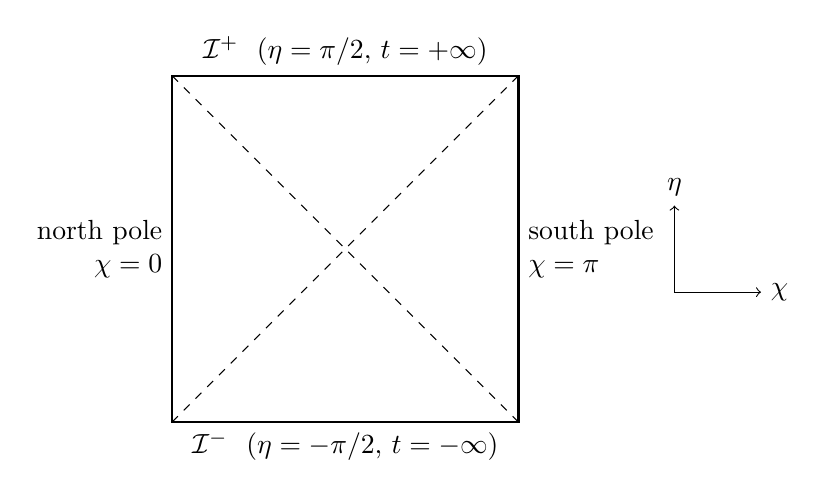
\begin{tikzpicture}[scale=1.1]
\draw[thick] (0,0) rectangle (4,4);
\draw[dashed] (0,0) -- (4,4);
\draw[dashed] (4,0) -- (0,4);
\node[above] at (2,4) {$\mathcal I^+$ \ ($\eta=\pi/2$, $t=+\infty$)};
\node[below] at (2,0) {$\mathcal I^-$ \ ($\eta=-\pi/2$, $t=-\infty$)};
\node[left,align=right] at (0,2) {north pole\\ $\chi=0$};
\node[right,align=left] at (4,2) {south pole\\ $\chi=\pi$};
\draw[->] (5.8,1.5) -- (5.8,2.5) node[above] {$\eta$};
\draw[->] (5.8,1.5) -- (6.8,1.5) node[right] {$\chi$};
\end{tikzpicture}
\end{center}
The dashed diagonals are light rays from the poles; e.g.\ the diagonal from $(\chi,\eta)=(\pi,-\pi/2)$ to $(0,\pi/2)$ is the cosmological event horizon of the observer at the north pole: since a light ray takes the full conformal time $\pi$ to cross from one pole to the other, an observer can never see the whole space---regions beyond the horizon are causally disconnected from them.

\section*{Question 5}
\textbf{a)} Under an infinitesimal diffeomorphism $h_{\mu\nu}\to h_{\mu\nu}+\partial_\mu\xi_\nu+\partial_\nu\xi_\mu$, so $\bh_{\mu\nu}\to\bh_{\mu\nu}+\partial_\mu\xi_\nu+\partial_\nu\xi_\mu-\eta_{\mu\nu}\partial^\rho\xi_\rho$ and
$\partial^\mu\bh_{\mu\nu}\to\partial^\mu\bh_{\mu\nu}+\Box\xi_\nu$. Choosing $\xi$ with $\Box\xi_\nu=-\partial^\mu\bh_{\mu\nu}$ (always solvable) achieves the Lorenz (de Donder) gauge
\[
\partial^\mu\bh_{\mu\nu}=0 .
\]
Then the second and third terms of the linearised equation vanish, leaving
\[
\Box\bh_{\mu\nu}\equiv\partial^\rho\partial_\rho\bh_{\mu\nu}=-16\pi G\,T_{\mu\nu}.
\]
In vacuum ($T_{\mu\nu}=0$) this is the wave equation $\Box\bh_{\mu\nu}=0$, whose solutions are superpositions of plane waves $\bh_{\mu\nu}=C_{\mu\nu}e^{ik_\rho x^\rho}$ with $k^\rho k_\rho=0$: perturbations of the metric propagate as waves at the speed of light. These are gravitational waves. (Residual gauge freedom with $\Box\xi=0$ allows the transverse--traceless gauge $h_{0\mu}=0$, $h=0$, $\partial^ih_{ij}=0$, leaving two physical polarisations $h_+,h_\times$.)

\textbf{b)} The full metric is $g_{\mu\nu}=\eta_{\mu\nu}+h_{\mu\nu}$:
\[
ds^2=-dt^2+\big(1+h_+(t-z)\big)dx^2+\big(1-h_+(t-z)\big)dy^2+dz^2 .
\]
\emph{Particles stay at fixed coordinates.} A particle initially at rest has $u^\mu=(1,0,0,0)$, and the geodesic equation gives
$\frac{du^i}{d\tau}=-\Gamma^i_{00}=-\tfrac12\eta^{ij}(2\partial_0h_{j0}-\partial_jh_{00})=0$ since $h_{0\mu}=0$. So in this (TT) gauge free test particles keep constant spatial coordinates; any physical effect shows up in the proper distance.

\emph{Particle on the $x$-axis.} At fixed $t$, along the path $y=z=0$, $0\le x\le L_x$, we have $ds^2=(1+h_+(t))dx^2$ (since $z=0$, $h_+(t-z)=h_+(t)$, independent of $x$). Thus
\[
\Delta s=\int_0^{L_x}\sqrt{1+h_+(t)}\,dx=L_x\sqrt{1+h_+(t)}\approx L_x\left(1+\tfrac12h_+(t)\right),
\]
to first order in $|h_+|\ll1$ (using $\sqrt{1+\epsilon}\approx1+\epsilon/2$).

\emph{Particle on the $y$-axis.} Along $x=z=0$, $0\le y\le L_y$: $ds^2=(1-h_+(t))dy^2$, so
\[
\Delta s=\int_0^{L_y}\sqrt{1-h_+(t)}\,dy=L_y\sqrt{1-h_+(t)}\approx L_y\left(1-\tfrac12h_+(t)\right).
\]
So as the wave passes, the $x$-separation is stretched while the $y$-separation is squeezed, and vice versa half a period later (the ``plus'' polarisation pattern).

\textbf{c)} \emph{Evolution of the binary.} The orbiting masses have a time-varying quadrupole moment, so they radiate gravitational waves at twice the orbital frequency, carrying away energy and angular momentum. Losing energy, the orbit shrinks; by Kepler's law the orbital frequency increases, which increases the radiated power ($P\propto \omega^{10/3}$), so the process runs away:
\begin{itemize}
\item \textbf{Inspiral:} a long phase in which the bodies slowly spiral together. The signal is a quasi-sinusoid whose frequency and amplitude both increase with time --- a ``chirp''. The rate of frequency increase is fixed by the chirp mass $\mathcal M=(m_1m_2)^{3/5}/(m_1+m_2)^{1/5}$, and the amplitude falls off as $1/(\text{distance})$.
\item \textbf{Merger:} when the separation becomes comparable to a few Schwarzschild radii, the bodies plunge together and coalesce (for black holes, horizons merge into one distorted horizon). This gives the peak amplitude and highest frequency, in the strongly nonlinear regime (requires numerical relativity).
\item \textbf{Ringdown:} the single distorted remnant black hole settles down to a stationary Kerr black hole by emitting quasi-normal modes: an exponentially damped sinusoid with a frequency and damping time set by the final mass and spin.
\end{itemize}

\begin{center}
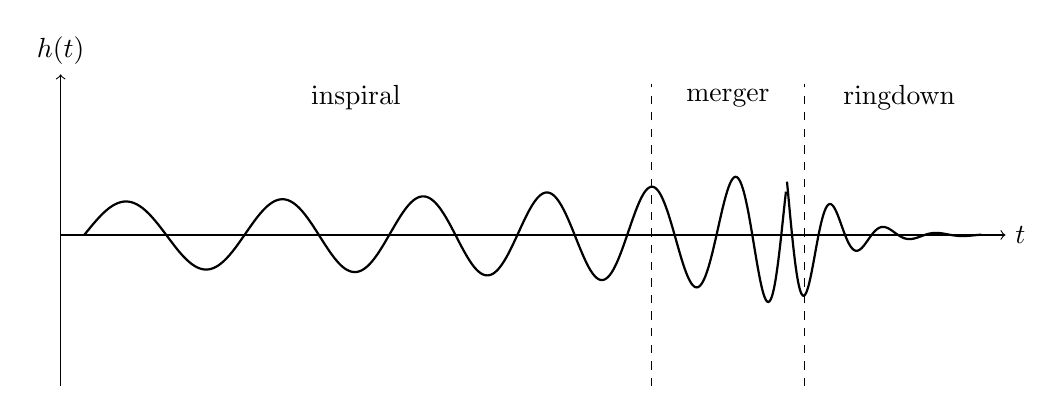
\begin{tikzpicture}[xscale=1.5,yscale=1.2]
\draw[->] (-6.2,0) -- (1.8,0) node[right] {$t$};
\draw[->] (-6.2,-1.6) -- (-6.2,1.7) node[above] {$h(t)$};
% inspiral chirp: tau = -x, phase ~ tau^{5/8}, amplitude ~ tau^{-1/4}
\draw[thick,domain=-6:-0.05,samples=600,smooth] plot (\x,{0.55*(-\x+0.15)^(-0.25)*sin(deg(14*(6.15^(0.625)-(-\x+0.15)^(0.625))))});
% ringdown
\draw[thick,domain=-0.05:1.6,samples=300,smooth] plot (\x,{1.0*exp(-3*(\x+0.05))*sin(deg(14*(6.15^(0.625)-0.1^(0.625)) + 14*(\x+0.05)))});
\draw[dashed] (-1.2,-1.6) -- (-1.2,1.6);
\draw[dashed] (0.1,-1.6) -- (0.1,1.6);
\node at (-3.7,1.45) {inspiral};
\node at (-0.55,1.45) {merger};
\node at (0.9,1.45) {ringdown};
\end{tikzpicture}
\end{center}

\emph{Detection.} LIGO is a Michelson interferometer with two perpendicular arms (length $L\approx4$\,km) along, say, the $x$ and $y$ axes, with mirrors suspended as freely falling test masses---exactly the configuration of part b). A wave like that of part b) changes the arm lengths in opposite senses, $\delta L_x/L=+\tfrac12h_+$, $\delta L_y/L=-\tfrac12h_+$, so the light round-trip times in the two arms differ by $\delta t\approx 2L h_+/c$ (to first order). This changes the relative phase of the recombined beams, so the intensity at the output (dark) port oscillates in step with $h_+(t)$. The detector output is thus directly proportional to the strain $h(t)$, and records the chirp sketched above: the inspiral frequency evolution gives the chirp mass, the peak marks the merger, and the ringdown frequency and damping time give the mass and spin of the final black hole. The tiny strains ($h\sim10^{-21}$) require extremely sensitive, long-baseline interferometry and several detectors to rule out local noise.

\end{document}
